\section{Instruction decoding}
The instruction decoding step occurs just after the instruction is fetched from memory. Its purpose is to identify the operation to be performed, generating control signals for subsequent stages. Its tasks also include detecting particular execution states where the pipeline has to be stalled or flushed.
Given the variety of its purposes, this block is furtherly broken down into several sub-units hierarchically:
\begin{itemize}
	\item Decoder
	\item Hazard Detection Unit (HZU)
	\item Branch Prediction Unit (BPU)
	\item Target address computation
	\item Register File
\end{itemize}

\subsection{Decoder}
The simplicity of RISC instruction sets consists in including few instructions that perform simple tasks. Furthermore, the instruction format is fixed, so as to allow the decoding circuitry to be as simple and fast as possible. Five types of instruction are defined in RISC-V, with the following types of fields that could be present depending on the actual format:
\begin{itemize}
	\item Opcode
	\item Specialized opcode fields for arithmetic operations (funct3 and funct7)
	\item Destination register
	\item Source registers (one, two or none)
	\item Immediate field, whose size and format varies across types
\end{itemize}
Since the position of each of these fields is fixed, they can be extracted into separate signals without detecting the instruction type first. After instruction decoding, the relevant fields are used and invalid signals corresponding to inexistent fields are just ignored.

The main task of this sub-unit is to drive control signals for execution, memory and write-back stages, which includes part of the ID stage itself given that data is written back to the register file.

The VHDL description consists in a combinational process whose sensitivity list includes the opcodes and the source registers. Based on \texttt{rs1} and \texttt{rs2}, this unit will resort to the hazard detection unit to handle the load-use data hazard occurring when the source operand is to be loaded from memory within the following two clock cycles. Under this circumstance, an operation that depends on such operand cannot proceed to the execution stage because it will be too early for the required data to be available of forwardable. Whenever the HZU runs into a load-use data hazard, the decoding step produces a NOP (no operation), meaning that all control signals are inactive and the instruction fetch stage is prompted to re-fetch the current instruction without updating \texttt{PC}. The normal execution flow proceeds as soon as the hazard is removed.

\begin{figure}[htb]
    \center
	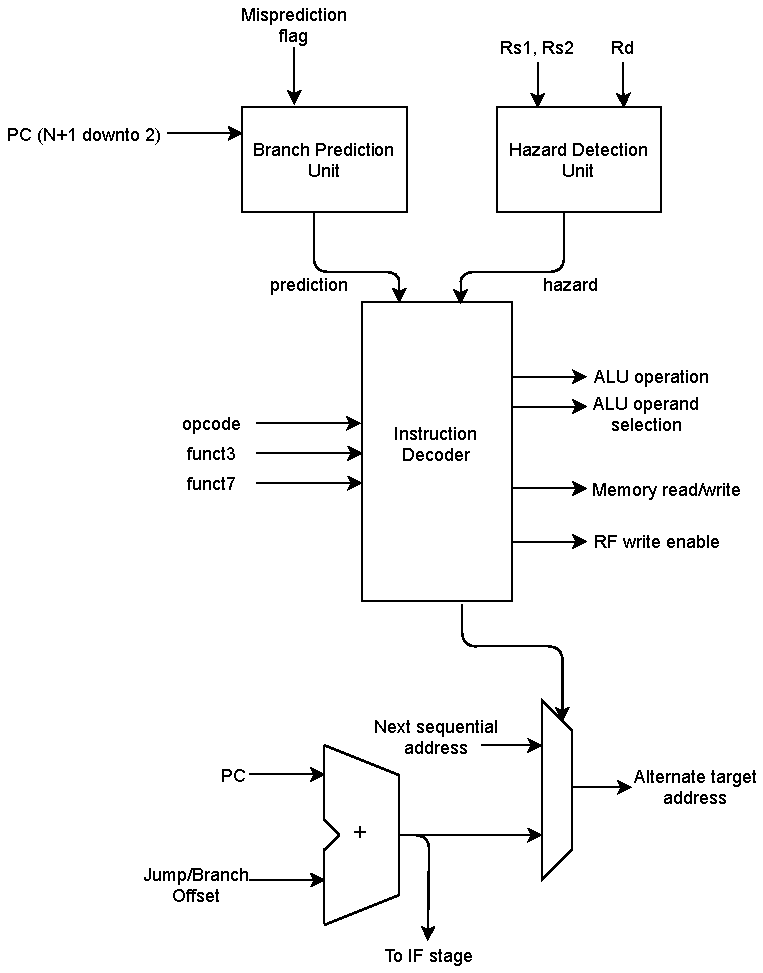
\includegraphics[width=0.6\textwidth]{./images/idstage.pdf}
	\caption{Instruction decoding stage with its sub-units}
	\label{fig:idstage}
\end{figure}

\subsection{Hazard Detection Unit} This subunit takes the source register indices and the \texttt{rd} signals (destination register name) both at the output of ID/EX and EX/MEM pipeline stages. If any of \texttt{rs1} or \texttt{rs2} is the same as \texttt{rd} and the corresponding data memory read enable signal is active, then the condition for a potential load-use data hazard is verified. The instruction decoder will trigger a NOP insertion after validating the hazard signal coming from this unit, which is effective only if the instruction depends on the data contained in the register involved in the hazard.


\subsection{Branch Prediction Unit} The purpose of this block is to estimate which is the most likely path that the execution will take in case of branch instruction. The actual outcome of the branch condition is known as soon as \texttt{beq} reaches the MEM stage, which happens with a two clock cycles delay. The BPU uses this outcome to update its internal state according to algorithms specifically designed to refine the prediction accuracy by collecting execution statistics.

In our implementation, branches are statically predicted to be taken, in a similar way as prediction schemes used in early microprocessors. The introduction of a BPU influences the timing of the processor. With a BPU, the pipeline is stalled upon decoding a \texttt{beq} for only one clock cycle if the branch is predicted, the minimum required to jump to a non-sequential address. The actual execution path as determined by checking the \texttt{Z} flag is compared to the prediction only two clock cycles later by combinational logic contained in the MEM stage. A misprediction causes the pipeline to be flushed (pipeline registers are reset to a \texttt{NOP} state) and the IF stage to jump to the alternative target address available in the EX/MEM pipeline register, which contains the alternative address computed in the ID stage.

A basic one-level scheme is the bimodal predictor, consisting in an array of 2-bit saturating counters addressed by part of the instruction address. Whenever a branch is decoded, the counter corresponding to its address is read, thus giving a 'taken' prediction when its value is greater than 1 and 'not-taken' otherwise. As soon as the real outcome of the branch is available the counter is incremented in case of a taken branch and decremented otherwise. This, in our implementation, occurs two cycles after decoding, when the branch is in the MEM stage. In general this delay, which affects the branch penalty to be paid in case of a flush, depends on the number of pipeline stages in between ID and MEM.


\subsection{Target address computation} This is accomplished simply by summing the offset specified in the instruction's immediate field (properly aligned and extended to 32 bits) to the current program counter. When the branch is predicted to be taken, this address is loaded in the pc and a jump takes place, with the next sequential address loaded in the alternative target address register. Otherwise, the TA is the alternative target address and the execution continues sequentially.

\subsection{Immediate} The immediate field is encoded differently depending on the instruction format. The ID stage takes care of aligning all the bits from the instruction word correctly and extending the sign bit to deliver a 32-bit immediate operand. This can take place after opcode decoding.

This is described in VHDL using a combinational \texttt{when-else} statement to synthesize a selection logic.

\subsection{Register file} As prescribed by the specifications, RV32I entails grouping 32 internal registers holding 32-bit data in a register file. \texttt{x0} denotes a location that always returns zero when read, thus making all write operations targeting it equivalent to not writing any data back.

The VHDL description of this sub-unit is that of a standard memory, with additional care taken to obtain the correct synthesis for the \texttt{x0} location, which might not correspond to a physical register.
